\documentclass[a4paper]{article}
\usepackage[utf8]{inputenc}
\usepackage[czech]{babel}
\usepackage[margin=13mm, tmargin=15mm, bmargin=12mm]{geometry}
\usepackage{multirow}
\usepackage{tikz}
\usetikzlibrary{calc}
\usepackage{chngpage}
\usepackage{tabularx}
\usepackage{fancyhdr}
\usepackage{mathptmx}
\usepackage{siunitx}
\usepackage{float}
\usepackage{longtable}
\usepackage{amsmath}

\renewcommand{\baselinestretch}{1.15}
\pagenumbering{gobble}
\pagestyle{fancy}
\renewcommand{\headrulewidth}{0pt}

\newcommand{\jmeno}{David Škrob, Tom\'{a}\v{s} N\'{a}zler}
\newcommand{\trida}{L3A}
\newcommand{\poradovecislo}{}
\newcommand{\nazevulohy}{Tranzistory}
\newcommand{\cisloulohy}{}
\newcommand{\predmet}{Technické měření}
\newcommand{\skupina}{}
\newcommand{\datummereni}{2.3.2022}
\newcommand{\datumodevzdani}{24.3.2022}
\newcommand{\klasifikace}{}
\begin{document}
\fancyhead{
\begin{tikzpicture} [overlay,remember picture]
       \draw
        ($ (current page.north west) + (1cm, -12mm) $)
        rectangle
        ($ (current page.south east) + (-1cm,12mm) $);
\end{tikzpicture}
}

\renewcommand{\arraystretch}{2}
\shorthandoff{-}

{
\begin{adjustwidth}[]{-3mm}{-3mm}
\centering
\vspace*{-7mm}
\begin{tabularx}{\linewidth}{l|X|p{3cm}}
\multirow{2}{25mm}{\centering SPŠ a VOŠ technická Brno, Sokolská 1} &
\textbf{LABORATORNÍ CVIČENÍ Z ELEKTROTECHNIKY} & Třída: \trida \\
\cline{2-3}
 & Jméno a příjmení: \jmeno & Poř. Číslo: \poradovecislo \\
\hline
\end{tabularx}

\begin{tabularx}{\linewidth}{X|p{3cm}}
Název úlohy: \nazevulohy & Číslo úlohy: \cisloulohy \\
\hline
Zkoušený předmět: \predmet & Skupina: \skupina \\
\hline
\end{tabularx}

\begin{tabularx}{\linewidth}{X|X|X}
Datum měření: \datummereni &  Datum odevzdání: \datumodevzdani &  Klasifikace: \klasifikace \\
\hline
\end{tabularx}

\end{adjustwidth}
}

\shorthandon{-}

\section*{Zadání}
Změřte následující voltampérové charakteristiky (VA) tranzistoru BC546B v zapojení se společným
emitorem. Použijte modul V-A Characteristics. Voltampérové charakteristiky v každém úkolu změřte
do jednoho grafu (použijte tlačítko Sequence).
\begin{enumerate}
	\item Změřte vstupní charakteristiky pro napětí $U_{CE}: 0 mV$, $20 mV$, $50 mV$, $100 mV$ podle schématu
	na obr. \ref{fig:mesh1}. Odpor $R_b$ použijte $1 k\Omega$. Kromě obrázku (obvyklý způsob) je uložte v datové formě
	(Zvolte Save, uložit jako typ Export do textového souboru. Ukládání dat funguje správně pouze
	při minimálním Zoom – zašedlá tlačítka ”
	mínus“. ).
	Hodnoty Output Ramp nastavte v rozmezí 0 až 10 $V$ a hodnotu Sense R nastavte na 1 $k\Omega$.
	V pracovním bodě $U_{CE} = 50 mV$ a $I_B = 5 mA$ z naměřených hodnot určete statický i dynamický
	vstupní odpor tranzistoru.
	Po přezkoušení správnosti zapojení a před zahájením měření přemostěte pomocí spojky ochrany
	b a c.
	\begin{figure}[H]
		\centering
		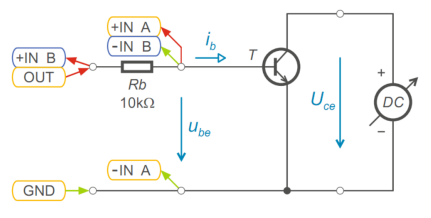
\includegraphics[width=0.75\textwidth]{schema1.png}
		\caption{Schéma k úkolu 1}
		\label{fig:mesh1}
	\end{figure}
	\item Změřte převodní charakteristiky pro napětí $U_{CE}$: 100 $mV$, 500 $mV$, 1000 $mV$, 2000 $mV$.
	Vyjděte ze schématu pro vstupní charakteristiky, do kolektorové větve zapojte rezistor 100 $\Omega$,
	paralelně k němu připojte sondy kanálu B. Do větve báze zapojte rezistor 1 k$\Omega$, paralelně k němu
	připojte sondy kanálu A.
	Hodnoty Output Ramp nastavte v rozmezí 0 až 10 $V$ a hodnotu Sense R nastavte na 100 $\Omega$.
	Kromě obrázku je opět uložte v datové formě (viz bod 1). Data je nutné zpracovat Excelu, protože
	RC2000 neumí měřit závislost dvou proudů. Pro přepočet naměřeného napětí na proud $I_B$ použijte
	Ohmův zákon a hodnotu odporu 1 k$\Omega$.
	Po přezkoušení správnosti zapojení a před zahájením měření přemostěte pomocí spojky ochrany
	b a c.
	\item Změřte výstupní charakteristiky pro napětí $U_{BE}$: 2000 $mV$, 4000 $mV$, 6000 $mV$, 8000 $mV$
	podle schématu na obr. \ref{fig:mesh2}.
	Kromě obrázku je také uložte v datové formě (viz bod 1). Změřte také multimetrem odpovídající
	klidové proudy báze $I_{B0}$.
	Hodnoty Output Ramp nastavte v rozmezí 0 až 10 $V$ a hodnotu Sense R nastavte na 100 $\Omega$.
	Po přezkoušení správnosti zapojení a před zahájením měření přemostěte pomocí spojky ochrany
	b a c.
	V pracovním bodě $U_{CE} = 1 V$ a $U_{BE} = 8000 mV$ z naměřených hodnot určete statický i dynamický
	výstupní odpor tranzistoru.
	\begin{figure}[H]
		\centering
		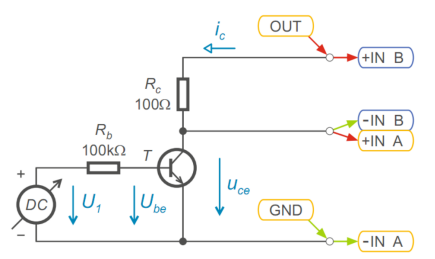
\includegraphics[width=0.75\textwidth]{schema2.png}
		\caption{Schéma k úloze 3}
		\label{fig:mesh2}
	\end{figure}
	\item Sestavte všechny naměřené charakteristiky do třech kvadrantů jednoho (velkého) grafu tak, jak
	se charakteristiky tranzistorů běžně zobrazují. Využijte Excel a uložená data.
\end{enumerate}
\section*{Teorie}
Chování tranzistoru ve větším rozsahu napětí a proudu popisují (při pomalých změnách veličin) nejlépe
statické charakteristiky, které se znázorňují graficky a vyjadřují vždy závislost dvou veličin, přičemž
třetí veličina se uvažuje jako parametr. Ze čtyř veličin $U_1, U_2, I_1$ a $I_2$ lze sestavit 4! = 24 různých soustav
charakteristik. Pro praxi jsou však důležité jen čtyři z nich, a to vždy jen v jednom kvadrantu. Proto se
často všechny čtyři zakreslují do jednoho grafu tak, že každá zabírá jeden kvadrant. V takovém tvaru
bývají charakteristiky uváděny také v katalogu výrobce.
Čtveřice používaných charakteristik je:\\
vstupní charakteristika (nakrátko)\\
$I_B = f(U_{BE}); U_{CE}= konst.$\\
výstupní charakteristika (naprázdno)\\
$I_C = f(U_{BE}); I_B= konst.$\\
proudová převodní charakteristika (nakrátko)\\
$I_C = f(I_B); U_{CE} = konst.$\\
zpětná napět’ová převodní charakteristika (naprázdno)\\
$U_{BE} = f(U_{CE}); I_B= konst.$\\
My budeme měřit první tři z nich.\\
\section*{Vypracování}
\begin{figure}[H]
	\centering
	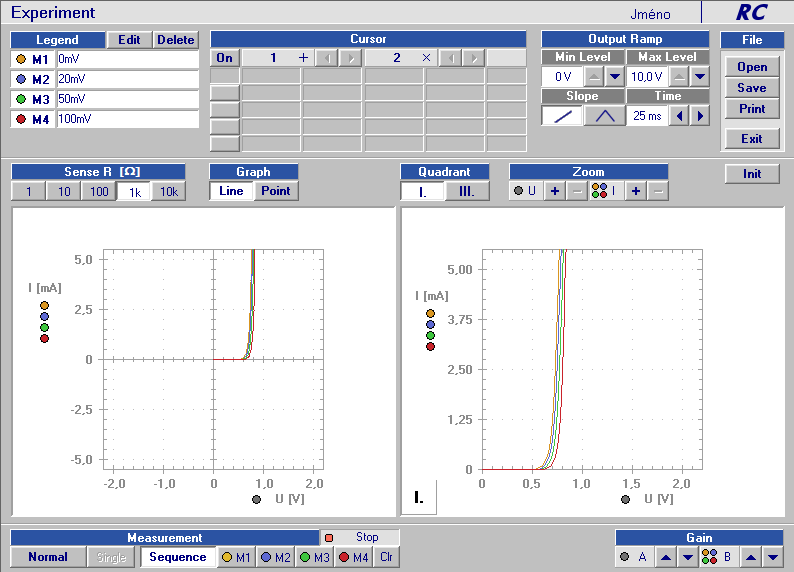
\includegraphics[width=0.9\textwidth]{tranzistory1.png}
	\caption{Vstupní charakteristiky}
\end{figure}
\begin{figure}[H]
	\centering
	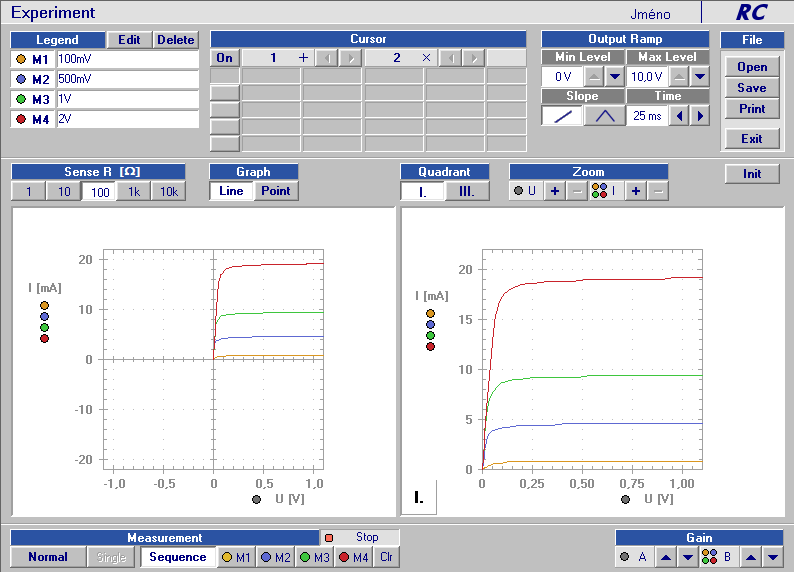
\includegraphics[width=0.9\textwidth]{tranzistory2.png}
	\caption{Převodní charakteristiky}
\end{figure}
\begin{figure}[H]
	\centering
	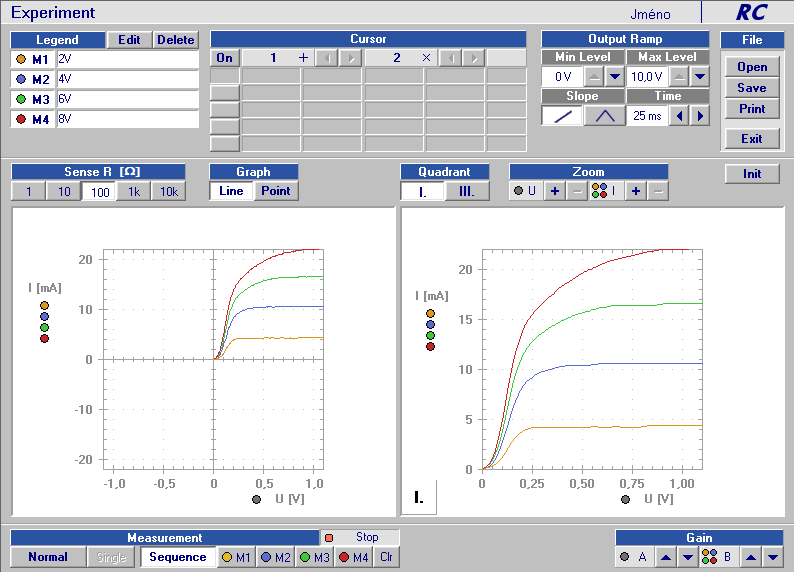
\includegraphics[width=0.9\textwidth]{tranzistory3.png}
	\caption{Výstupní charakteristiky}
\end{figure}
\begin{figure}[H]
	\centering
\begin{minipage}[b]{0.49\textwidth}
	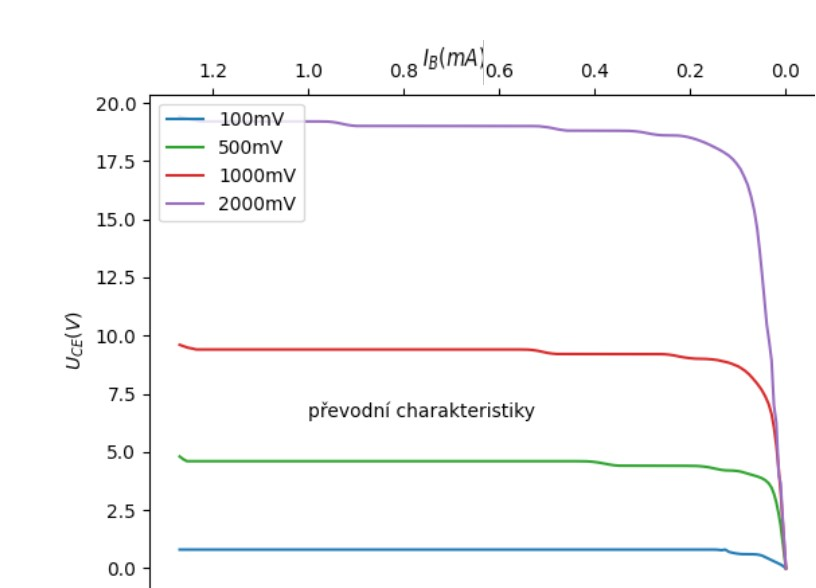
\includegraphics[width=\textwidth]{2.jpg}
\end{minipage}
\begin{minipage}[b]{0.435\textwidth}
	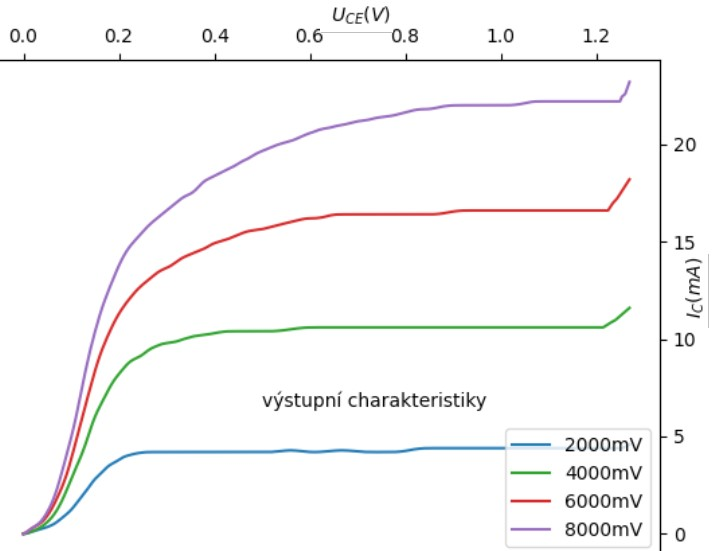
\includegraphics[width=\textwidth]{3_2.jpg}
\end{minipage}
\\
	\centering
	\hspace*{.99cm}
	\begin{minipage}[b]{0.48\textwidth}
		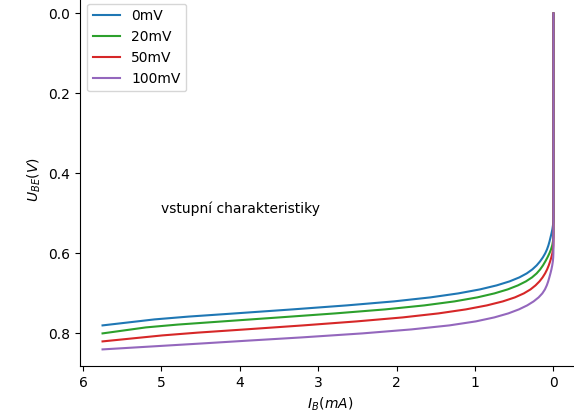
\includegraphics[width=\textwidth]{Figure_1.png}
	\end{minipage}
	\hfill
	\begin{minipage}[b]{0.45\textwidth}
		\hfill
	\end{minipage}
	\caption{Graf dle bodu 4 v zadání}
\end{figure}
Pro příklad 1\\
Klidový odpor vypočítáme dle ohmova zákona
$U_{BE} =0,805  V $; $I_B = 4,9866 mA  \implies R = \frac{0,805 V}{4,9866 mA} = 161.43 \Omega $%prehozeny obracene to je proste retardovany
. Pro dynamický odpor platí $R =\lim_{\Delta I \to 0}  \frac{\Delta U}{\Delta I}$\\
\begin{minipage}{0.3\textwidth}
\begin{tabular}{|c|c|} 
	\hline
	$U_{BE}$ & $I_B$ \\ \hline
	0,798 $V$ & 4,5332 $mA$ \\ 
	0,805 $V$ & 4,9866 $mA$ \\ 
	0,820 $V$ & 5,7500 $mA$ \\ 
	\hline
\end{tabular}
\end{minipage}
\begin{minipage}{0.6\textwidth}
\begin{math}
	\Delta U_{BE} =0,820 V - 0,798 V = 0,022V \\
	\Delta I_B =5,7500 mA- 4,5332 mA = 1,2168 mA \\
	\implies R_{dyn} = \SI{18,08}{\ohm}\\
\end{math}\\
\end{minipage}\\
\iffalse
\begin{figure}[H]
	\centering
	\begin{minipage}[b]{0.33\textwidth}
		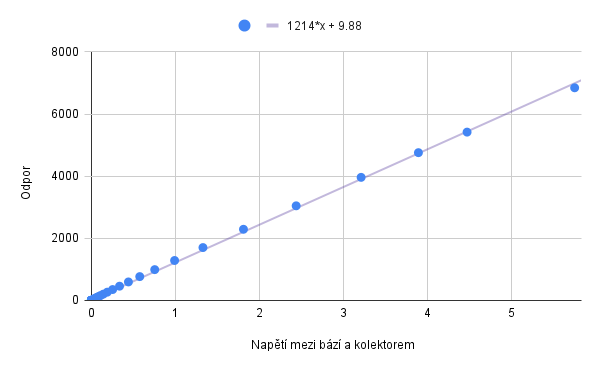
\includegraphics[width=\textwidth]{chart.png}
	\end{minipage}
	\begin{minipage}[b]{0.33\textwidth}
		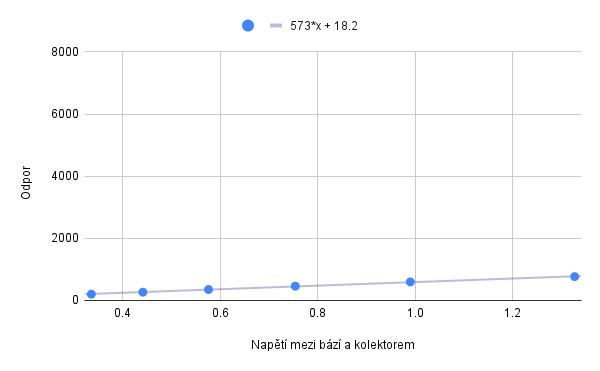
\includegraphics[width=\textwidth]{chart (1).png}
	\end{minipage}
	\begin{minipage}[b]{0.33\textwidth}
		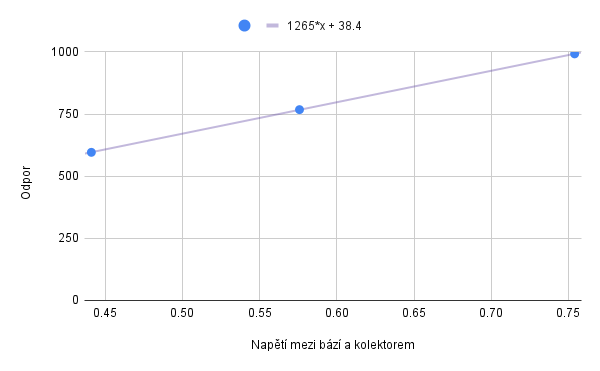
\includegraphics[width=\textwidth]{chart (2).png}
	\end{minipage}
	\caption{Graf postupného snižování $\Delta I$}
\end{figure}
\fi
%Dle grafu potom vidíme, že dynamický odpor v pracovním bodě$U_{BE} =0,5758  V $; $I_B = 0,75 mA$ $\implies R \approx 1200\Omega$\\%dynamicky odpor je derivace proudu dle napeti, ne odporu dle napeti....
\vspace*{0.5cm}\\
Pro příklad 3 potom\\
Klidový odpor vypočítáme dle ohmova zákona% OPRAVIT
$U_{CE} = 1 V $; $I_C =45,54 mA  \implies R = \frac{1V}{45,54 mA} = \SI{21,96}{\ohm} $
\iffalse
\begin{figure}[h]
	\centering
	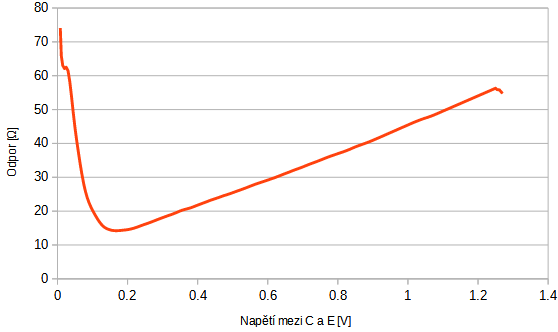
\includegraphics[width=0.75\textwidth]{rezist.png}
	\caption{Závislost $R$ na $U_{CE}$ (příklad 3)}
	\label{fig:mesh3}
\end{figure}
\fi
Pro dynamický odpor platí $R =\lim_{\Delta I \to 0}  \frac{\Delta U}{\Delta I}$\\
\begin{minipage}{0.3\textwidth}
	\begin{tabular}{|c|c|}
		\hline
		$U_{CE}$ & $I_C$ \\ \hline
		\SI{0,98}{\volt} & \SI{22,000}{\milli\ampere} \\%% 45 je odpor - musim sem hodit proud
		\SI{1,00}{\volt} & \SI{22,000}{\milli\ampere} \\
		\SI{1,02}{\volt} & \SI{22,006}{\milli\ampere} \\
		\hline
	\end{tabular}
\end{minipage}
\begin{minipage}{0.6\textwidth}
	\begin{math}
		\Delta U_{CE} =\SI{1.02}{\volt} - \SI{0,98}{\volt} = \SI{0,04}{\volt} \\
		\Delta I_C =\SI{22,000}{\milli\ampere}- \SI{22,006}{\milli\ampere} = \SI{0,006}{\milli\ampere} \\
		\implies R_{dyn} = \SI{6666}{\ohm}\\
	\end{math}\\
\end{minipage}\\
\iffalse
\begin{figure}[H]
	\centering
	\begin{minipage}[b]{0.33\textwidth}
		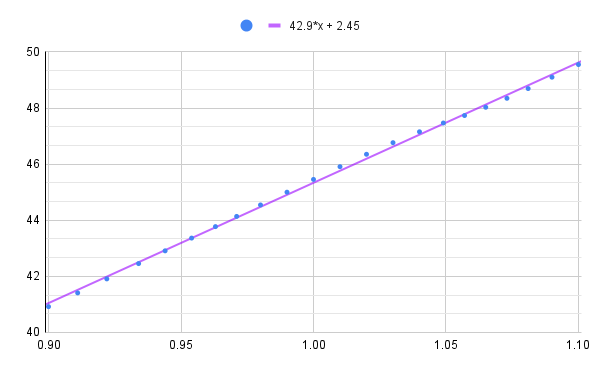
\includegraphics[width=\textwidth]{d1.png}
	\end{minipage}
	\begin{minipage}[b]{0.33\textwidth}
		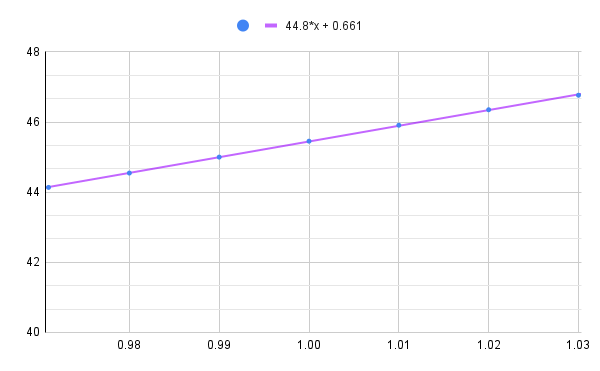
\includegraphics[width=\textwidth]{d2.png}
	\end{minipage}
	\begin{minipage}[b]{0.33\textwidth}
		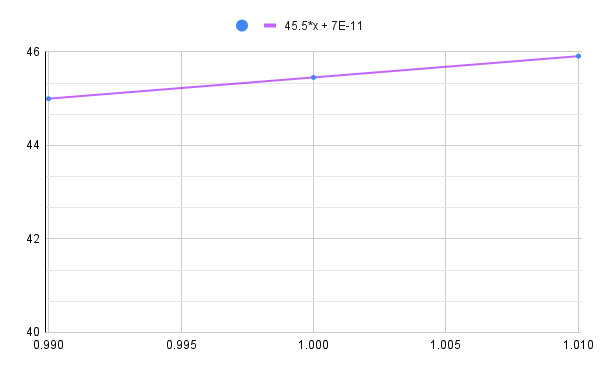
\includegraphics[width=\textwidth]{d3.png}
	\end{minipage}
	\caption{Graf postupného snižování $\Delta I$}
\end{figure}
\fi
%Dle grafu potom vidíme, že dynamický odpor v pracovním bodě $U_{CE} = 1 V $; $I_C = 22 mA $ $\implies R \approx 45,5\Omega$
\section*{Závěr}
No zaver si napis sam :D
\iffalse
Měření dopadlo tak jak jsme čekali, obr. \ref{fig:mesh3}. odpovídá tomu, že přechod PN musíme zmenšit vyprázdněnou vrstvu,takže překonáváme velký odpor, následně je odpor prakticky lineární, což značí, že PN přechod je správně vyrobený, a při vyšším než difuzním napětí prochází proud.\fi  
\vfill
\section*{Použité pomůcky:}
\begin{tabularx}{\linewidth}{c|c|c|c}
	Přístroj – pomůcka & Typ & Rozsah (pouze analogové)
	& Poznámka \\
	\hline
	RC 2000 & Digitální && V režimu V-A Characteristics
\end{tabularx}
\end{document}